\section{LO2: Visual Perception}
Visual perception is a critical factor in data visualization, as it directly impacts how the audience interprets the data being presented \cite{wareInformationVisualizationPerception2013a}. Understanding the basics of visual perception can significantly aid in creating more effective visualizations.

\subsection{Perceptual Variables and Their Impact}
Jacques Bertin identified several visual variables that are pivotal in shaping how we perceive data visualizations \cite{bertinSemiologyGraphicsDiagrams2011}. These include size, shape, lightness/value, orientation, texture, location, hue, saturation/intensity, and arrangement. Each of these variables has its own set of strengths and weaknesses that can either enhance or compromise the quality of a data visualization. A comprehensive list of these variables and their strengths and weaknesses is presented in the table (Table \ref{tab:bertin_variables}).

\begin{table}[h]
    \centering
    \renewcommand{\arraystretch}{1.5} % Increase row height
    \begin{tabularx}{\textwidth}{|X|X|X|}
\hline
\textbf{Variable}    & \textbf{Strengths}                       & \textbf{Weaknesses}                           \\
\hline \hline
Size                 & Easily distinguishable                   & Limited scalability                           \\
\hline
Shape                & Good for categorization                  & Limited set of easily distinguishable shapes  \\
\hline
Lightness/Value      & Wide range                               & Affected by surrounding colors                \\
\hline
Orientation          & Effective for differentiation            & Can be confusing if too many orientations     \\
\hline
Texture              & Effective for background differentiation & Limited set and may be confusing              \\
\hline
Location             & Fundamental to spatial analysis          & Requires good layout                          \\
\hline
Hue                  & Excellent for categories                 & Limited number of easily distinguishable hues \\
\hline
Saturation/Intensity & Good for indicating importance           & Can overwhelm if used excessively             \\
\hline
Arrangement          & Effective for organization               & Requires thoughtful design                    \\
\hline
    \end{tabularx}
    \caption{Bertin's Visual Variables}
    \label{tab:bertin_variables}
\end{table}

Understanding and effectively using these variables can greatly improve the clarity and impact of a visualization. The scatter plot (Figure \ref{fig:lo2_scatter_plot}) demonstrates the interplay of size, hue, and spatial positioning to represent different data dimensions. The size of each point corresponds to a country's population, the hue indicates its continent, and the axes show GDP per capita and life expectancy. This visualization exemplifies how combining various visual variables can effectively convey multi-faceted data relationships.

\begin{figure}[h]
    \centering
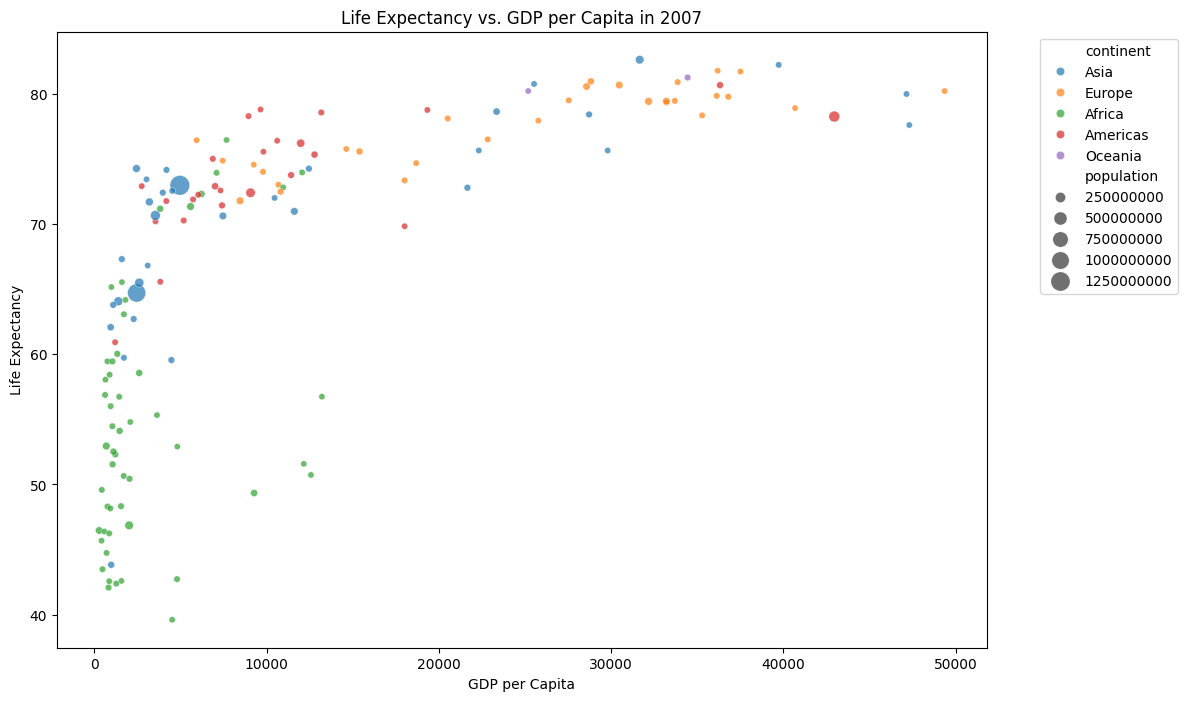
\includegraphics[width=0.8\textwidth]{images/plots/lo2_life_exp_vs_gdp_cap_2007.png}
    \caption{Scatter Plot of Life Expectancy vs. GDP per Capita (2007): Demonstrating the Integration of Size, Hue, and Spatial Positioning in Data Visualization.}
    \label{fig:lo2_scatter_plot}
\end{figure}

\subsection{Gestalt Principles in Visualization}
Gestalt psychology offers valuable insights into how humans perceive visual elements, which can be leveraged to improve data visualization \cite{kohlerGestaltPsychology1929}. Important principles include figure-ground, proximity, closure, and common fate. Incorporating these principles in data visualization enhances the interpretability and effectiveness of visual representations, leading to better comprehension and decision-making.

\subsubsection{Figure-Ground}
The figure-ground principle aids in distinguishing the object (figure) from the background (ground), which is particularly crucial in map visualizations.

The map visualization (Figure \ref{fig:lo2_scatter_plot}) demonstrates the figure-ground principle, where specific countries (highlighted in blue) are made prominent against a uniform background. This contrast aids in distinguishing these countries from the rest of the world, emphasizing their data in the global context. Such visual distinction is essential in complex visual fields to focus attention on key areas.

\begin{figure}[h]
    \centering
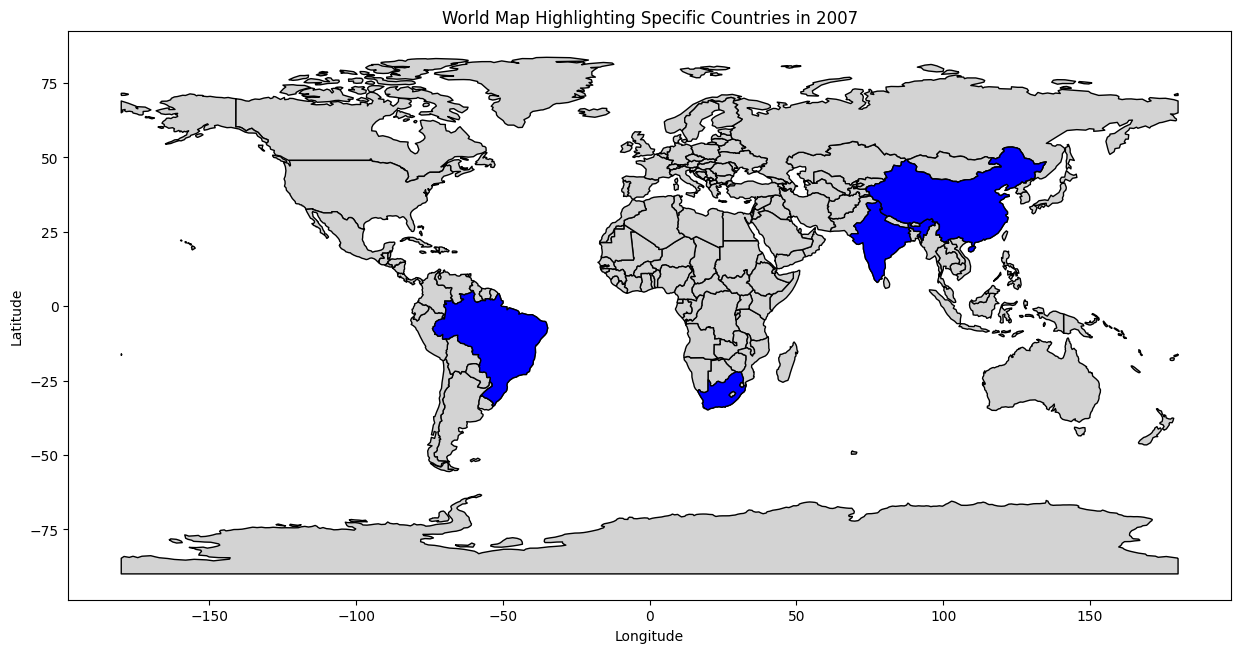
\includegraphics[width=0.8\textwidth]{images/plots/lo2_world_map_highlight_countries_2007.png}
    \caption{Map Highlighting Specific Countries (2007): An Illustration of the Figure-Ground Principle in Geographic Data Representation.}
    \label{fig:lo2_map}
\end{figure}


\subsubsection{Proximity}

The figure-ground principle helps viewers distinguish an object (figure) from its surroundings (ground). This is crucial in visualizations like maps, where identifying specific data points or regions against a complex background is necessary. For example, in a scatter plot, proximity can indicate clusters of related data. Studies show that proximity facilitates the extraction of ensemble statistics, enhancing visual memory in arrays \cite{imMeanSizeUnit2014}. Proximity's influence is significant in assigning features to clusters based on the input proximity matrix \cite{scottFeatureGroupingRelocalisation1990}. It also has a substantial impact on the perceived unity of groups in visualizations \cite{promannEffectProximitySocial2018}.

\subsubsection{Closure}

The principle of closure aids in interpreting incomplete visual information as complete forms. For example, in line graphs with missing data points, viewers can still perceive the overall trend. Closure can affect the interpretation of data visualizations, like in infrared spectral library search performance \cite{harringtonClosureEffectsInfrared1987}. In human visual perception, closure processes help organize the world by filling in gaps in stimulation, leading to the perception of whole objects \cite{chenInvestigationClosureProcess1998}.

The line graph (Figure \ref{fig:lo2_line_chart_w_gaps}), depicting India's life expectancy over time with intentional gaps in data, exemplifies the closure principle. Despite missing data points for certain years, the viewer perceives a continuous trend line, illustrating how the human mind tends to complete incomplete visual information.

\begin{figure}[h]
    \centering
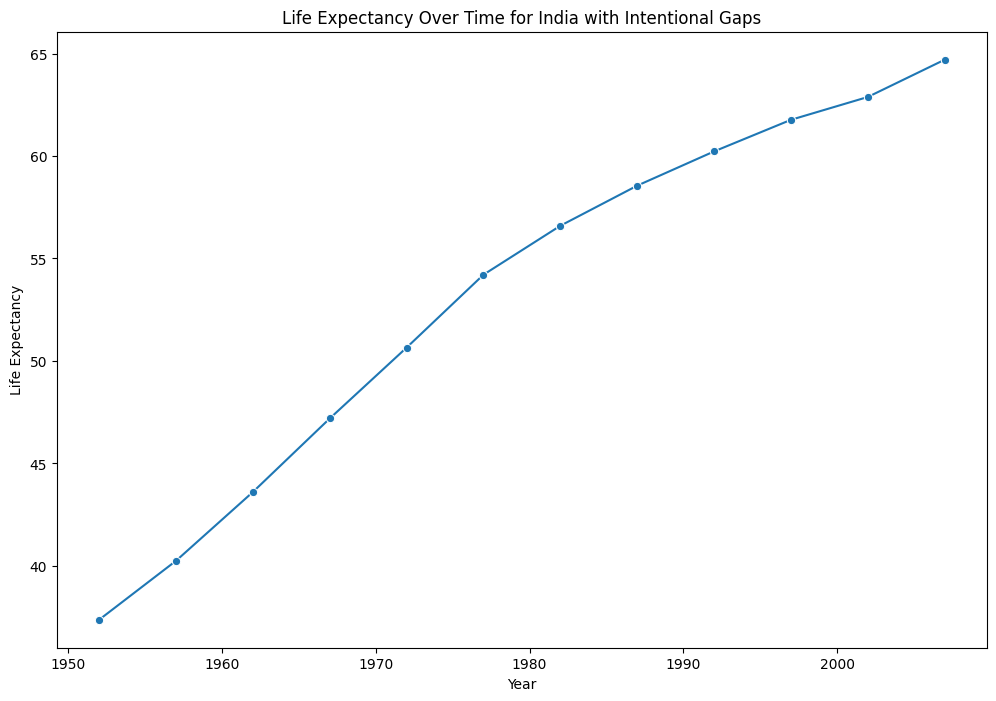
\includegraphics[width=0.8\textwidth]{images/plots/lo2_life_exp_over_time_with_gaps_India.png}
    \caption{Line Graph Showing India's Life Expectancy Over Time with Gaps: A Demonstration of the Closure Principle in Visual Data Interpretation.}
    \label{fig:lo2_line_chart_w_gaps}
\end{figure}

\subsubsection{Common Fate}

Common fate, where elements moving in the same direction are perceived as part of the same group, is vital for animations in data visualizations. Research shows that common fate involves attentional selection of motion direction, limiting the formation of more than one group at a time \cite{levinthalCommonFateGroupingFeature2011}. It's also utilized in motion-based segmentation methods for improving detection accuracy \cite{kopacsiCommonFateBased2019}.